% This is LLNCS.DEM the demonstration file of
% the LaTeX macro package from Springer-Verlag
% for Lecture Notes in Computer Science,
% version 2.4 for LaTeX2e as of 16. April 2010
%
\documentclass{llncs}
%
\usepackage{graphicx}
\usepackage{makeidx}  % allows for indexgeneration
%
\begin{document}
%
\frontmatter          % for the preliminaries
%
%\pagestyle{headings}  % switches on printing of running heads
%
%
\title{When is QVTc/QVTr check-before-enforce sound?}
%
\titlerunning{QVT check-before-enforce soundness}  % abbreviated title (for running head)
%                                     also used for the TOC unless
%                                     \toctitle is used
%
\author{Edward D. Willink}
%
\authorrunning{Edward D. Willink} % abbreviated author list (for running head)
%
%%%% list of authors for the TOC (use if author list has to be modified)
\tocauthor{Edward Willink}
%
\institute{Willink Transformations Ltd., Reading, UK,\\
\email{ed \_at\_ willink.me.uk}
}

\maketitle              % typeset the title of the contribution

\begin{abstract}
QVTr offers a check-before-enforce execution mode that has come in for some legitimate criticism. I have emailed to a few authors to suggest that I think that the mode should be removed from the specification and left as an optimization offered by good tools. In this discussion paper, I identify why check-before-enforce is unsound in the general case, but can be sound in many practical cases.
\end{abstract}
%

\section{Enforce}

QVTr and QVTc may perform an enforce execution to fully create an output model from an input model. This is shown in a fairly minimal form in Fig~\ref{fig:Enforce}

\begin{figure}[h]
	\centering
	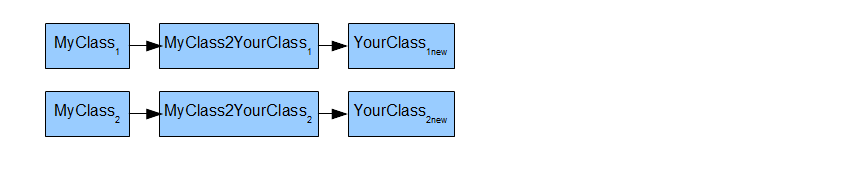
\includegraphics[width=1.0\textwidth]{Enforce.png}
	\caption{Enforce execution.}
	\label{fig:Enforce}
\end{figure}

Two instances of MyClass are transformed via the intermediate trace class MyClass2YourClass to two instances of YourClass; there are no class properties.

Perhaps the most important characteristic of any M2M language is traceability which enables the creation of a graph-structured output model to resolve input-to-output mappings to establish the graph cross-links. Without traceability we can only transform to tree-structures.

In QVTr and QVTc the internal traceability of many transformation languages is reified by the trace classes that map the input bindings to the output bindings. MyClass2YourClass is the trace class with a rather trivial input binding to a MyClass and an output binding to an YourClass. With two inputs mapped to two outputs there are two trace class instances.

A trace instance is uniquely identified by its input bindings. Less obviously, even in a unidirectional scenario, a trace instance is also uniquely identified by its output bindings.

\section{Check-After-Enforce}

An important M2M use case is ``is-output-up-to-date-with-input" or ``has-the-input-changed-significantly". Both of these may be used as a guard to determine whether some downstream consequences of a changed output are necessary. 

Naively we could perform a check-after-enforce as shown in Fig~\ref{fig:CheckAfterEnforce}

\begin{figure}[h]
	\centering
	\includegraphics[width=1.0\textwidth]{CheckAfterEnforce.png}
	\caption{CheckAfterEnforce execution.}
	\label{fig:CheckAfterEnforce}
\end{figure}

We need to determine whether there is a permutation of YourClass\textsubscript{new} which supports a pairwise equivalence of YourClass\textsubscript{x,old} and YourClass\textsubscript{y,new}.

Clearly no such permutation exists if the size of YourClass\textsubscript{new} is not the same as the size of YourClass\textsubscript{old}.

\section{Check-Before-Enforce}

Performing a full execution and incurring all the inconvenience of creating a full YourClass\textsubscript{new} is undesirable if all that is required is a simple true/false result. QVTc/QVTr therefore offers a more efficient form of checkonly execution. And since unnecessary execution in general is undesirable, QVTc/QVTr directs that checkonly should be performed as a guard for any enforce execution to avoid the costs of a redundant enforce. This checkonly is therefore called check-before-enforce. We can wrap up this new form of execution as shown in Fig~\ref{fig:CheckBeforeEnforce}

\begin{figure}[h]
	\centering
	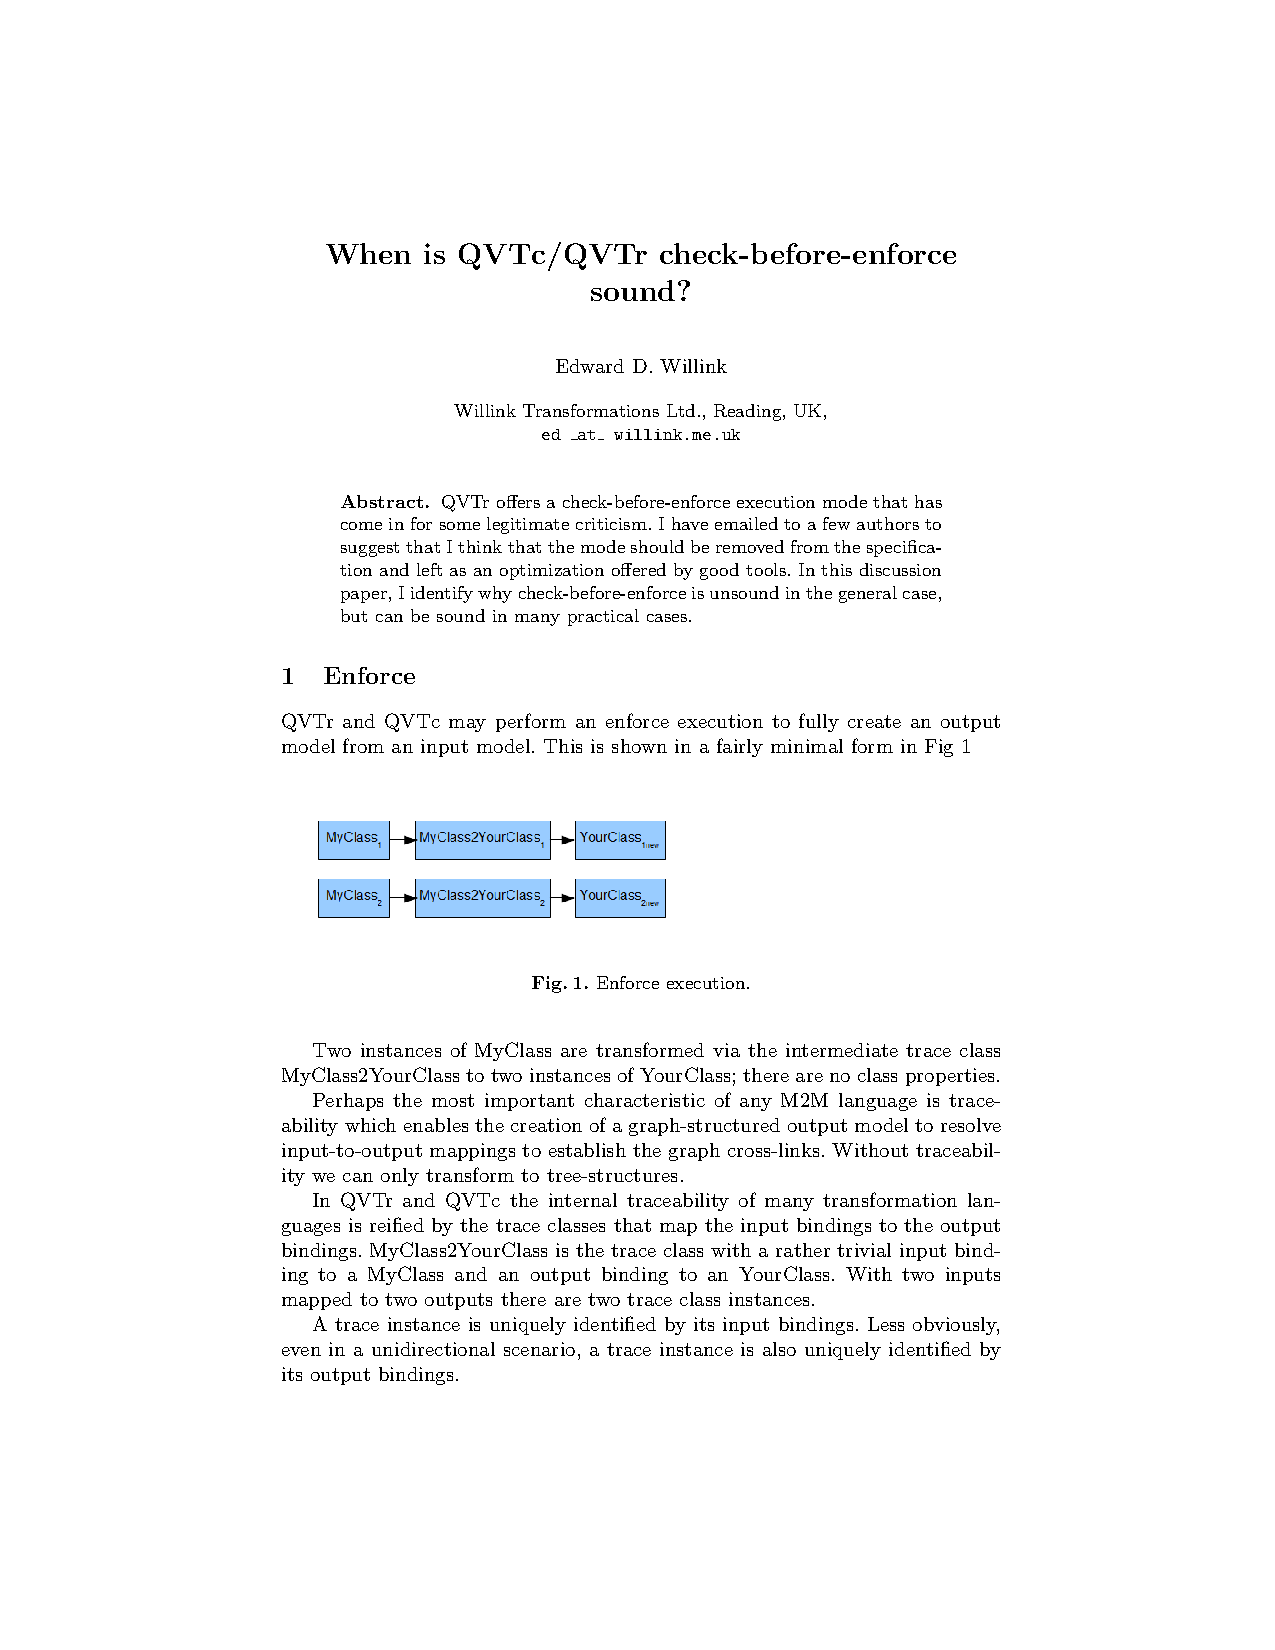
\includegraphics[width=1.0\textwidth]{CheckBeforeEnforce.png}
	\caption{CheckBeforeEnforce execution.}
	\label{fig:CheckBeforeEnforce}
\end{figure}

Not a problem. The Check-Before-Enforce Compare box works the magic.

Since check-before-enforce is a mandatory guard for enforce, the cascade of check-before-enforce followed by check-after-enforce must yield precisely the same result as check-after-enforce by itself.

This implies that for a given input model I, enforce execution may result in a set of alternative good-enough models G\footnote{Ideally G would be a single model, but due to accidental or deliberate vagueness in the use of ordered/unique collections, operations such as asSequence(), or iterations such as any() there may be some indeterminism leading to models that are good-enough.}. Conversely there is a universe of all possible output models A of which G is necessarily a subset. The universe of all possible models excluding the good-enough models is a set of bad output models B that cannot be the result of a transformation from I.

We expect that both check-before-enforce and check-after-enforce return
\begin{itemize}
	\item true, if the actual output model O is one of the good-enough models G.
	\item false, if the actual output model O is one of the bad models B.
\end{itemize}

\section{Unsound Check-Before-Enforce}

A simple implementation of the Check-Before-Enforce Compare box magic is provided by Appendix B.1 of the QVT specification~\cite{QVT-1.3}. It iterates over the input elements to check that it matches an output. It makes no use of trace elements and so does not ensure that outputs also correspond to inputs.

Perdita~\cite{Stevens-game} has identified that this doesn't work as shown in Fig~\ref{fig:UnsoundCheckBeforeEnforce}

\begin{figure}[h]
	\centering
	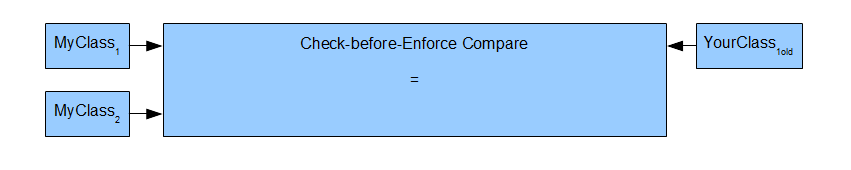
\includegraphics[width=1.0\textwidth]{UnsoundCheckBeforeEnforce.png}
	\caption{Unsound CheckBeforeEnforce execution.}
	\label{fig:UnsoundCheckBeforeEnforce}
\end{figure}

When considering each MyClass element it is possible to find a YourClass element that compares, but since this is a local decision without trace instances, the same YourClass element can be used to satisfy the match of multiple MyClass elements. check-before-enforce can therefore return true when check-after-enforce returns false.

\section{Sound Check-Before-Enforce}

The problem with the unsound check-before-enforce is that throwing away all the inconvenience of trace and output model element construction eliminates the critical unique and existence characteristics of the trace elements. We could attempt a sound check-before-enforce as shown in Fig~\ref{fig:SoundCheckBeforeEnforce}

\begin{figure}[h]
	\centering
	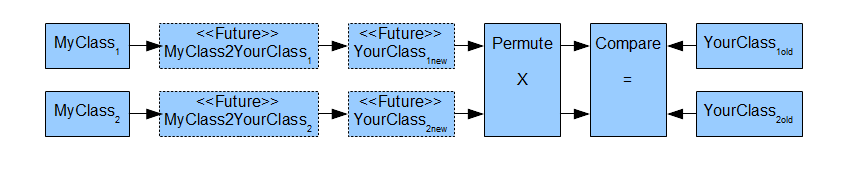
\includegraphics[width=1.0\textwidth]{SoundCheckBeforeEnforce.png}
	\caption{Sound CheckBeforeEnforce execution.}
	\label{fig:SoundCheckBeforeEnforce}
\end{figure}

We migrate the inconvenient trace/output construction costs to some to-be-designed form of future object so that we can perform the requisite global permutation and comparison of future YourClass\textsubscript{new} elements against the YourClass\textsubscript{old} elements. In the general case, for which the traces are essential for uniqueness and existence, it is not clear that replacement of MyClass2YourClass elements by future-MyClass2YourClass elements achieves anything. It may be possible to modify the permutation to work directly between MyClass2YourClass elements and YourClass\textsubscript{old} elements and so use each MyClass2YourClass as its future YourClass\textsubscript{new}. A sound check-after-enforce may therefore defer the output class creation until the check failure requires the enforce to repair the output creating those output elements that cannot be matched with existing outputs and deleting existing output elements that are not `created'.

\section{Sound Check-After-Enforce simplification}

When can check-after-enforce be simplified to a check-before-enforce?

a) When the global permutation can be simplified to a local selection.

This is possible if there is a pair of operations such as id(MyClass) and id(YourClass) that yield distinct DataType values for each distinct MyClass or YourClass, but yield the same DataType value for corresponding MyClass and YourClass. The simplest example is an id operation that just returns a name property that is globally unique. Slightly more complicated is a qualified name that is hierarchically unique. When an id function is available\footnote{QVTr provides keys that can be regarded as an operation yielding a unique value from an output element. A key is not useful for id purposes since there is no relationship between an input and output key and because keys do not work usefully in the presence of inheritance hierarchies.}, input and output models may be independently analyzed to identify id2MyClass and id2YourClass maps that facilitate checking consistency of the output graph cross-links.

b) When the trace class instances do not enforce uniqueness.

The trace instance is a simple input-to-output mapping, it can be optimised away as a simple id and a pair of id2input, id2output maps. However for more complex mappings involving multiple inputs, the complexity of multi-dimensional ids probably exceeds the complexity of the direct trace classes.

Given the significant limitations on the soundness of check-before-enforce, check-before-enforce should not be a mandatory guard for an enforce execution. Rather implementations should be free to choose to implement 
\begin{itemize}
	\item no check-before-enforce; just check-after-enforce
	\item no check-before-enforce; check-after-enforce variant of enforce
	\item check-before-enforce when valid; otherwise check-after-enforce
\end{itemize}

\section{Conclusion}

check-before-enforce is unsound unless
\begin{itemize}
	\item every mapping has a single input and output class.
	\item every input and output class has a unique identity property or operation.
\end{itemize}
check-before-enforce should be an optional facility


%
% ---- Bibliography ----
%
\begin{thebibliography}{}

\bibitem{Stevens-game}
Stevens, P : A simple game-theoretic approach to checkonly QVT-Relations,
Software and Systems Modeling 12,January 2009, pp. 165–180

\bibitem{QVT-1.3}
OMG. Meta Object Facility (MOF) 2.0 Query/View/Transformation Specification, Version 1.3.
OMG Document Number: formal/2016-06-03, April 2016.

\end{thebibliography}
\end{document}
